\documentclass[12pt]{article}
\usepackage{graphicx} % Required for inserting images
\usepackage{mathtools}
\usepackage{amsmath}
\usepackage{gvv-book}
\usepackage{gvv}
\usepackage[shortlabels]{enumitem}
\usepackage{multicol}

\title{\textbf{12.330}}
\author{\textbf{EE25BTECH11004 - Aditya Appana}}
\date{October 12, 2025}
\renewcommand{\labelenumi}{\Alph{enumi})}
\begin{document}

\maketitle

\section*{Question}
If a weight of $\vec{P}= 100N$ is supported by two massless strings connected to the walls
as shown in the figure, the value of $T_1$ is \rule{1.5cm}{0.15mm} N. 
\begin{figure}[H]
    \centering
    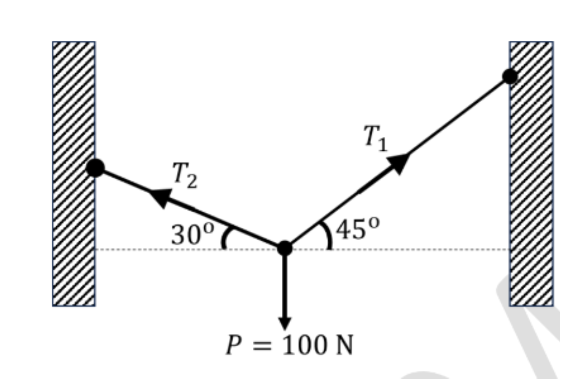
\includegraphics[width=0.4\columnwidth]{Figs/123301.png}
    \caption{Figure}
    \label{fig:placeholder}
\end{figure}

\section*{Solution}
\begin{align}
\vec{T_1} + \vec{T_2} = -\vec{P}\\
\vec{T_1} = \norm{T_1}\myvec{\cos 45 \degree \\ \sin 45 \degree}\\
\vec{T_2} = \norm{T_2}\myvec{\cos 180-30 \degree \\ \sin 180-30 \degree} =\norm{T_2}\myvec{\cos 150 \degree \\ \sin 150 \degree} \\
\vec{P} = -\norm{P}\myvec{\cos -90 \degree \\ \sin -90 \degree} = -100\myvec{\cos (-90 \degree) \\ \sin (-90 \degree)}
\end{align}
Therefore:
\begin{align}
    \norm{T_1}\myvec{\frac{1}{\sqrt{2}}\\ \frac{1}{\sqrt{2}}} + \norm{T_2}\myvec{-\frac{\sqrt{3}}{2} \\ \frac{1}{2}} = 100\myvec{0\\1} \\
    \myvec{\frac{1}{\sqrt{2}} & -\frac{\sqrt{3}}{2}\\  \frac{1}{\sqrt{2}} & \frac{1}{2}}\myvec{\norm{T_1} \\ \norm{T_2}} = \myvec{0 \\ 100}
\end{align}\\
Organising the data into an augmented matrix and obtaining RREF:
\begin{align}
\myaugvec{2}{ \frac{1}{\sqrt{2}} & -\frac{\sqrt{3}}{2} & 0\\  \frac{1}{\sqrt{2}} & \frac{1}{2} & 100}\xrightarrow{\text{$R_2$ \rightarrow $R_2- R_1$}}
\myaugvec{2}{ \frac{1}{\sqrt{2}} & -\frac{\sqrt{3}}{2} & 0\\ 0 & \frac{1}{2} +\frac{\sqrt{3}}{2} & 100}\xrightarrow{\text{$R_1$ \rightarrow $\sqrt{2}R_1$}}
\myaugvec{2}{ 1& -\sqrt{6} & 0\\  0 & \frac{1}{2} +\frac{\sqrt{3}}{2} & 100}
\end{align}
\begin{align}
    \norm{T_2} = \frac{200}{1+\sqrt{3}} = 73.205N\\
    \norm{T_1} = \frac{\sqrt{3}}{\sqrt{2}}\norm{T_2} = 89.658N
\end{align}


\begin{figure}[H]
    \centering
    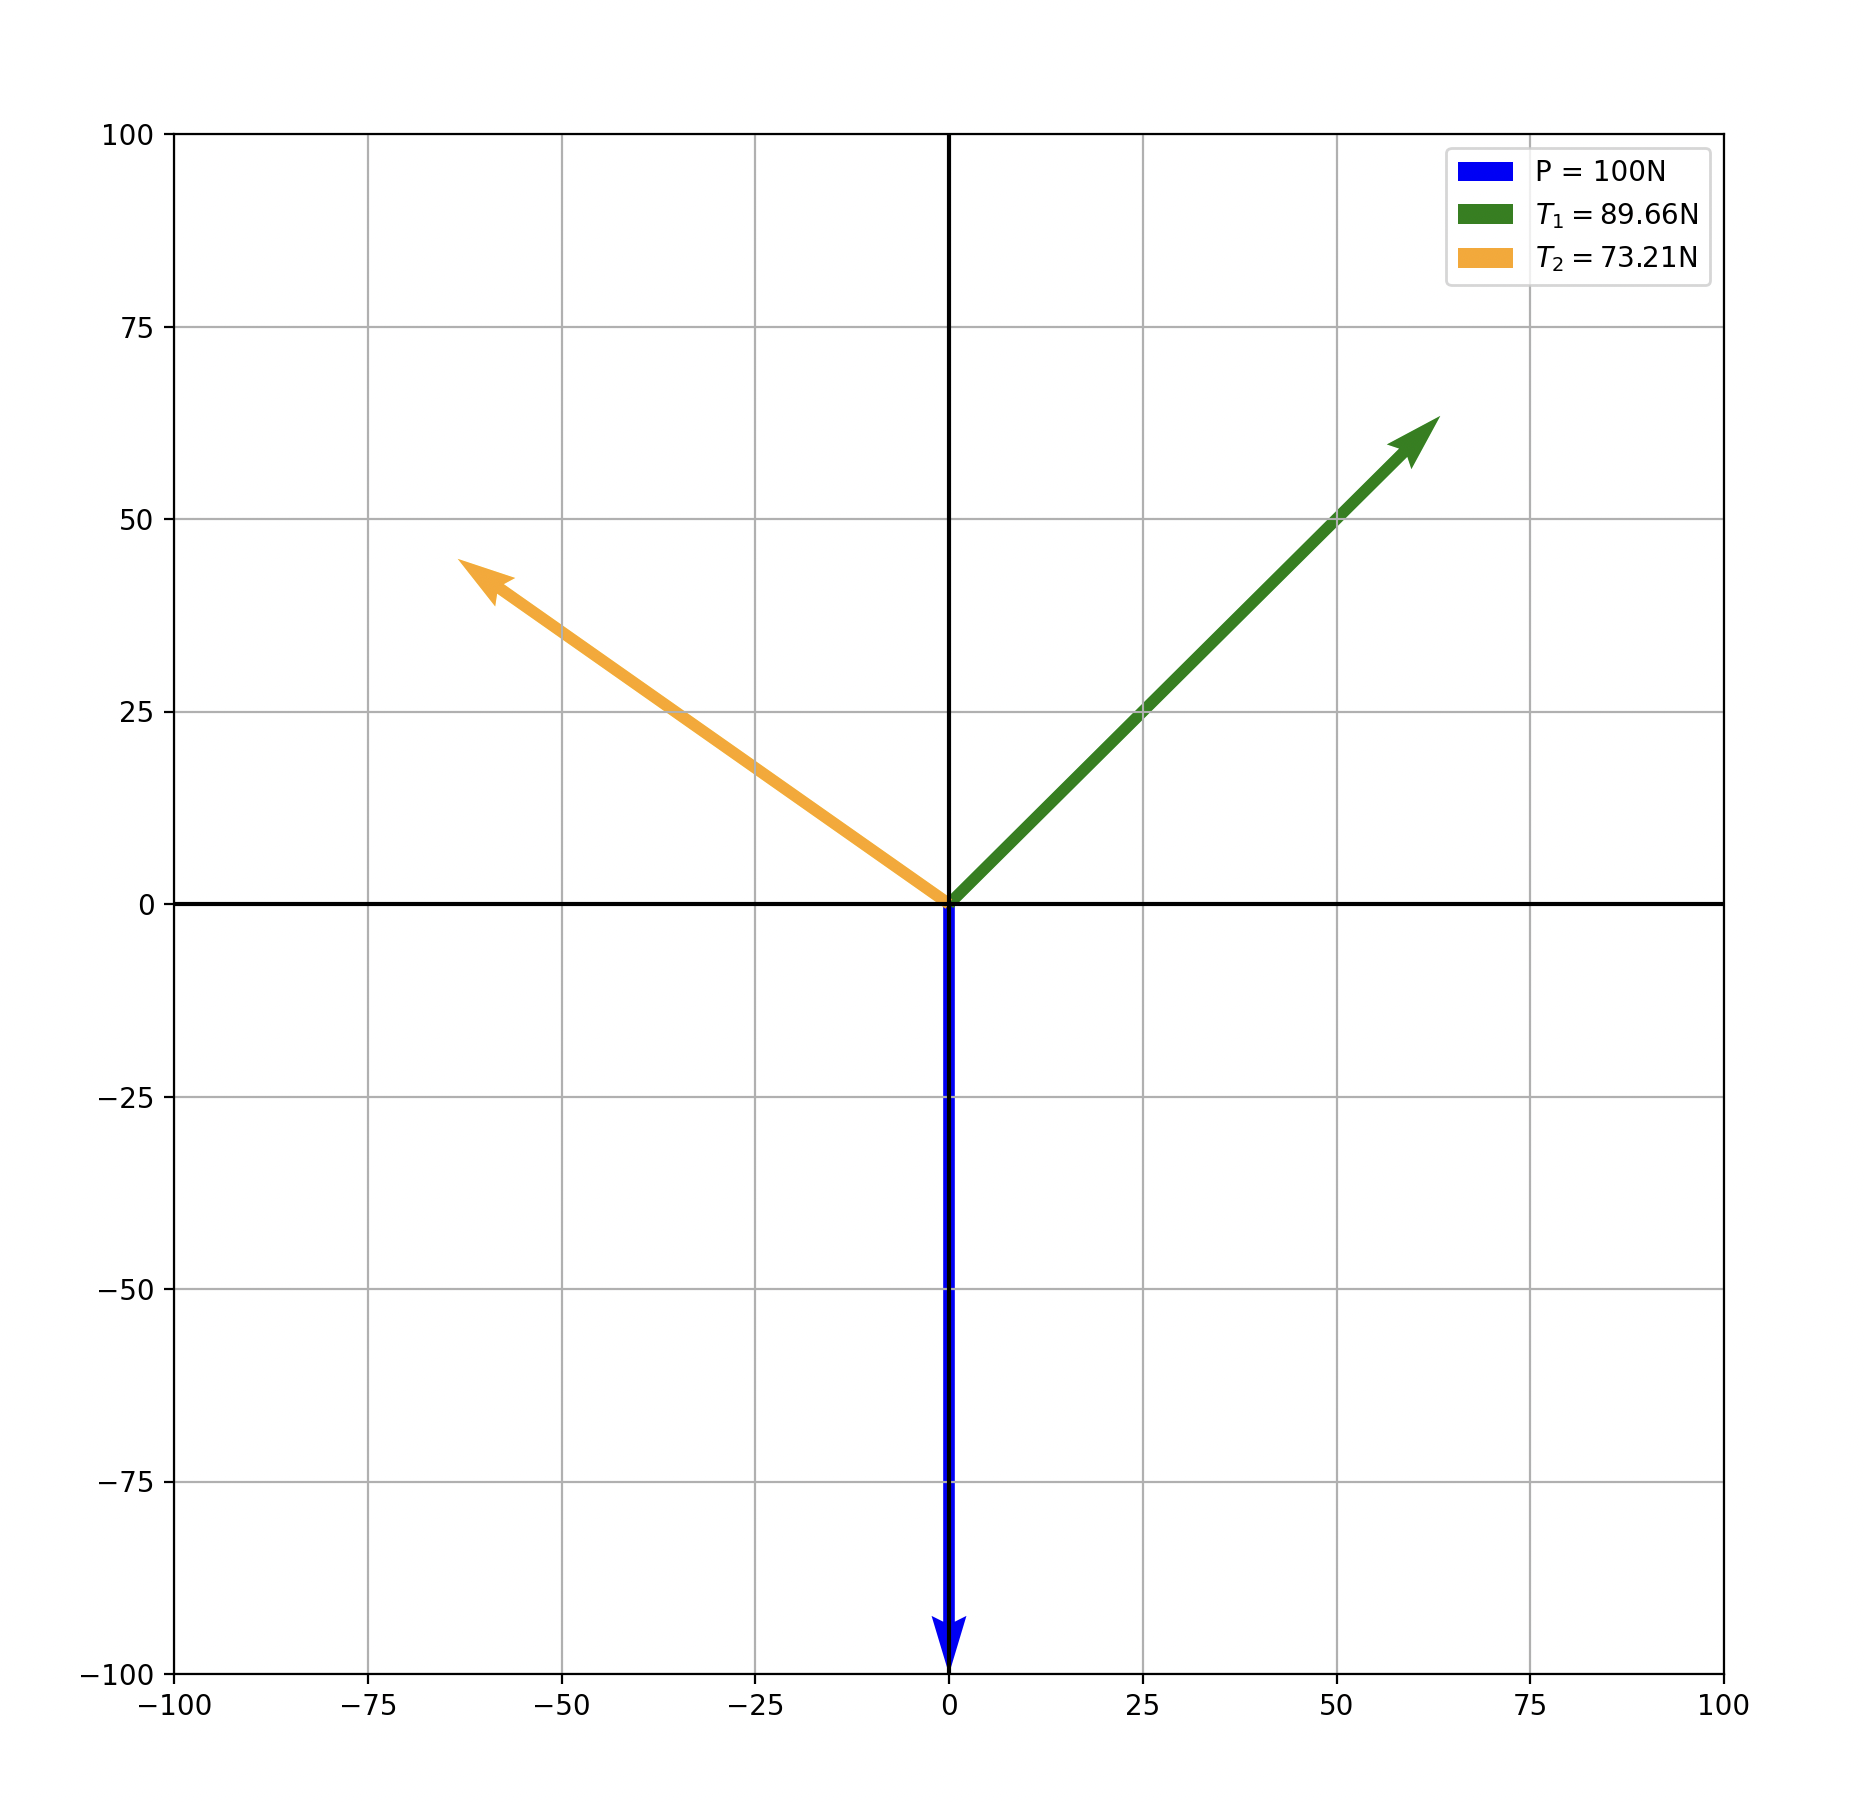
\includegraphics[width=0.6\columnwidth]{Figs/123302.png}
    \caption{Plot}
    \label{fig:placeholder}
\end{figure}
\end{document}
